\documentclass[11pt, a4paper]{article}
% Shared preamble for the methodology and validation reports.
%
% siunitx is loaded conditionally. It is standard in TeX Live and MacTeX, but
% absent from minimal Debian installations, and these documents must compile in
% continuous integration as well as on a workstation. The fallbacks reproduce
% only the commands used here.
\usepackage[a4paper, margin=25mm]{geometry}
\usepackage{amsmath}
\usepackage{booktabs}
\usepackage{tikz}
\usepackage{pgfplots}
\usepackage{subcaption}
\usepackage{graphicx}
\usepackage[hidelinks]{hyperref}

\usetikzlibrary{arrows.meta, positioning}
\pgfplotsset{compat=1.18}

% A conditional is used rather than the false branch of \IfFileExists because
% a macro parameter (#1) written inside another macro's argument is consumed
% during expansion, producing "Illegal parameter number".
\newif\ifhassiunitx
\IfFileExists{siunitx.sty}{\hassiunitxtrue}{\hassiunitxfalse}

\ifhassiunitx
  \usepackage{siunitx}
  \sisetup{detect-all, per-mode=symbol}
\else
  \typeout{NOTE: siunitx unavailable; using minimal fallbacks.}
  \providecommand{\num}[1]{\ensuremath{#1}}
  \providecommand{\si}[1]{\ensuremath{\mathrm{#1}}}
  \providecommand{\qty}[2]{\ensuremath{#1\,\mathrm{#2}}}
  \providecommand{\degree}{^{\circ}}
\fi

\newcommand{\code}[1]{\texttt{#1}}
\setlength{\parskip}{0.4em}
\setlength{\parindent}{0pt}


\title{Relief Forge Tools: Methodology}
\author{Mesh reconstruction and fabrication validation}
\date{}

\begin{document}
\maketitle

\begin{abstract}
This document describes the processing pipeline that converts image-derived
triangle meshes into dimensionally scaled solids suitable for small-scale
casting and additive manufacturing. The reconstruction model is treated as one
interchangeable mesh source; the subject of this document is the geometry
processing and verification applied to its output, which is independent of how
the mesh was produced.
\end{abstract}

\section{Overview}

The pipeline is a linear sequence with one optional stage
(Figure~\ref{fig:pipeline}). Only the generation stage depends on a
reconstruction model; every subsequent stage operates on triangle arrays and is
identical regardless of the mesh source. Meshes from a scanner, from CAD
export, or from a different generative model pass through the same code.

\begin{figure}[h]
  \centering
  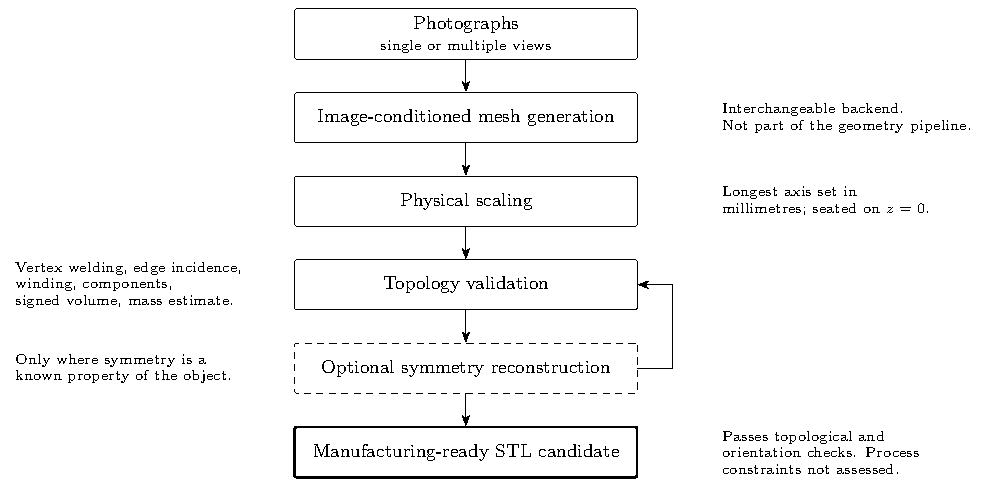
\includegraphics[width=0.92\textwidth]{generated/pipeline.pdf}
  \caption{Processing pipeline. The dashed stage is optional and triggers
  revalidation. Generation is the only stage requiring a model, GPU or network
  access.}
  \label{fig:pipeline}
\end{figure}

\section{Input preprocessing}

Inputs are one or more photographs of a single object. Background removal is
applied by default, isolating the subject from its surroundings before
inference.

Single-view input leaves the geometry of unobserved surfaces unconstrained: a
photograph records one side of an object, and any reconstruction of the
remainder is inferred rather than measured. Supplying additional views
constrains the reconstruction directly and is the most effective available
means of reducing that ambiguity. The pipeline accepts an arbitrary number of
views; the backend determines how many it uses.

\section{Mesh generation}

Generation is delegated to a backend implementing the \code{MeshGenerator}
interface. A backend accepts preprocessed images and returns a triangle array
in arbitrary units. Backends are selected by name at run time and registered
through a decorator, so adding a reconstruction model requires implementing one
class and no changes to any downstream stage.

Two properties of the interface matter for the rest of the pipeline. First, the
returned mesh is in arbitrary units and carries no physical scale, which
Section~\ref{sec:scaling} resolves. Second, the returned mesh is not assumed to
be valid: it may contain boundary edges, inverted normals or detached
fragments, and is subjected to the same validation as any other input.

No model weights are distributed with this software. Backends retrieve
third-party checkpoints on first use under those projects' own licence terms,
which differ from the licence of this repository.

\section{Physical scaling}
\label{sec:scaling}

Let $\mathbf{p}_{\min}$ and $\mathbf{p}_{\max}$ be the componentwise extrema of
all vertex positions, and let $L$ be the largest component of
$\mathbf{p}_{\max} - \mathbf{p}_{\min}$. For a target longest dimension
$L_{\mathrm{target}}$ in millimetres, every vertex is scaled by
$s = L_{\mathrm{target}} / L$.

The scaled mesh is then translated so that it is centred in $x$ and $y$ and its
minimum $z$ lies on the build plane:
%
\begin{equation}
  \mathbf{t} =
  \left(
    -\tfrac{1}{2}\left(x_{\min} + x_{\max}\right),\;
    -\tfrac{1}{2}\left(y_{\min} + y_{\max}\right),\;
    -z_{\min}
  \right)
\end{equation}
%
after scaling. This is the convention expected by slicers and by casting
service bureaux, and it makes the reported bounding box directly comparable to
a caliper measurement of the finished part.

\section{STL reconstruction}

The STL format stores three independent vertex positions per triangle and
provides no index buffer. A file describing a closed solid is therefore
byte-indistinguishable from one describing unconnected triangles, and no
topological question can be answered until coincident vertices have been
identified.

Vertex welding resolves this. Positions are snapped to a grid of spacing
$\varepsilon = \delta \cdot d$, where $d$ is the length of the bounding-box
diagonal and $\delta$ is a relative tolerance with default $10^{-6}$. Scaling
the tolerance with the model keeps its behaviour consistent across part sizes:
an absolute tolerance appropriate for a \qty{3}{mm} setting would be far too
coarse for a \qty{300}{mm} sculpture, and vice versa. Snapped positions are
deduplicated, producing a vertex array and an index array that preserves the
original winding order.

Two further format details are handled explicitly. Format detection compares
the declared triangle count against the file length rather than testing for a
leading \code{solid} keyword, since many binary writers emit that string.
Facet normals recorded in the file are discarded on read and recomputed from
winding on write, because stored normals frequently disagree with the geometry
they accompany.

\section{Topology analysis}

Each triangle $(v_0, v_1, v_2)$ contributes three directed edges: $(v_0,v_1)$,
$(v_1,v_2)$ and $(v_2,v_0)$. On a closed surface with globally consistent
winding, every directed edge occurs exactly once, and its reverse occurs
exactly once. Departures from this identify the defect rather than merely
reporting failure:

\begin{itemize}
  \item \textbf{Boundary edge}: incident to one triangle. The surface is open.
  \item \textbf{Non-manifold edge}: incident to more than two triangles. The
        surface self-intersects or contains an internal partition.
  \item \textbf{Inconsistently wound edge}: incident to two triangles that
        traverse it in the same direction, so neighbours disagree about which
        side faces outward.
  \item \textbf{Degenerate edge}: both endpoints weld to one vertex.
\end{itemize}

Connectivity is computed separately by union-find over triangle corners. A
single solid yields one component; higher counts indicate detached fragments,
which for generated meshes usually means floating debris.

Genus is not constrained. A washer with a through hole has Euler characteristic
$\chi = 0$ rather than $2$ and is entirely valid, so no check assumes a
simply connected surface.

\section{Symmetry reconstruction}

Where bilateral symmetry is a known property of the object, one half of the
mesh may be discarded and replaced by the reflection of the other. This is
useful when one side was captured or reconstructed more cleanly than the other.

The mesh is clipped against an axis-aligned plane by Sutherland--Hodgman
clipping applied per triangle; triangles crossing the plane yield a
quadrilateral or triangle, which is fan-triangulated. The retained half is then
reflected across the plane, and its winding reversed, since reflection inverts
handedness and would otherwise leave every mirrored normal pointing inward.

The clipped boundary lies exactly on the plane and is deliberately left open.
The reflected copy has an identical boundary, so welding the two halves closes
the seam without cap geometry.

Symmetric parts routinely have vertices lying exactly on their own mirror
plane, which produces three degenerate cases. A triangle lying wholly in the
plane would be duplicated by its own mirror image, creating a doubled interior
wall, and is discarded. A triangle on the discarded side touching the plane at
a single vertex clips to a zero-area sliver, removed by an area threshold. An
intersection computed at a vertex already on the plane repeats that point in
the output polygon, so consecutive duplicates are collapsed. Without all three,
the mirrored result is not manifold.

\textbf{Applicability.} Bilateral symmetry is not universally valid and nothing
in the software can verify it. Where the assumption holds, the operation
removes error; where it does not, it destroys real asymmetric geometry.
Reflecting front-to-back has a considerably weaker justification than
reflecting left-to-right, since a surface reconstructed from a single viewpoint
carries no information about the reverse side, and a mirrored back is
fabricated rather than recovered.

\begin{figure}[h]
  \centering
  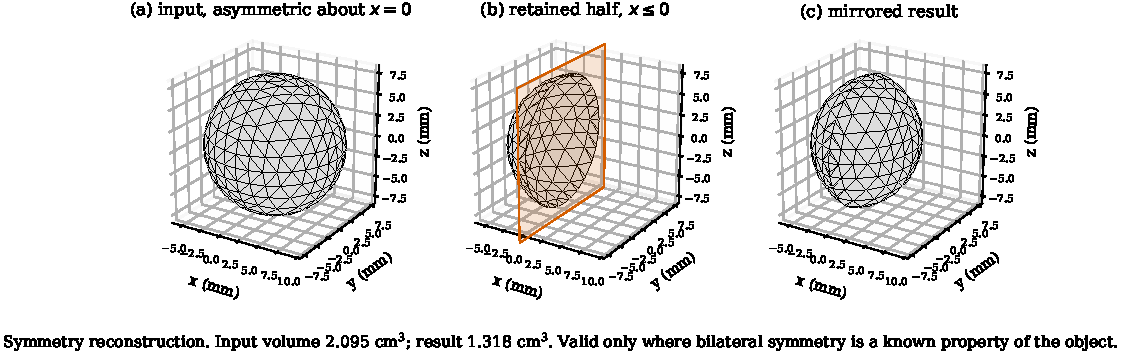
\includegraphics[width=\textwidth]{../figures/generated/fig_symmetry_operation.pdf}
  \caption{Symmetry reconstruction on a solid positioned asymmetrically about
  the cut plane. Camera and axis limits are identical in all three panels.}
  \label{fig:symmetry}
\end{figure}

\section{Material estimation}

Volume follows from the divergence theorem. For a closed surface of $N$
triangles with corners $\mathbf{a}_i$, $\mathbf{b}_i$, $\mathbf{c}_i$:
%
\begin{equation}
  V = \frac{1}{6} \sum_{i=1}^{N}
      \mathbf{a}_i \cdot \left( \mathbf{b}_i \times \mathbf{c}_i \right)
  \label{eq:volume}
\end{equation}
%
The sign of $V$ is positive when triangles are wound counter-clockwise as seen
from outside, so Equation~\ref{eq:volume} simultaneously measures volume and
tests global orientation. It is meaningful only on a closed surface; on an open
one the result depends on the choice of origin.

Triangle area, summed for total surface area, is
%
\begin{equation}
  A_i = \frac{1}{2}
        \left\| (\mathbf{b}_i - \mathbf{a}_i) \times
                (\mathbf{c}_i - \mathbf{a}_i) \right\|
  \label{eq:area}
\end{equation}
%
and estimated cast mass for a material of density $\rho$ is
%
\begin{equation}
  m = \rho \, |V|
  \label{eq:mass}
\end{equation}

Equation~\ref{eq:mass} assumes a fully dense solid. It excludes sprue,
flashing, and shrinkage, and the densities used are nominal values for common
alloys whose exact composition varies between suppliers. The estimate is
intended for comparing candidate geometries and anticipating material cost, not
for certifying a finished part.

\section{Interpretation of results}

A mesh passes this repository's checks when it has no boundary edges, no
non-manifold edges, no degenerate edges, consistent local winding, positive
signed volume, and the expected connected-component count.

Passing establishes that the mesh is a closed, coherently oriented solid. It
does not assess minimum wall thickness, unsupported overhangs, printer
tolerances, casting shrinkage, trapped volumes, or any constraint specific to a
manufacturing process. Those remain the responsibility of the operator and of
process-specific software.

\end{document}
